\documentclass[border=40pt]{standalone}
\usepackage{tikz}
\usepackage{pgfplots}
\usepackage{amsfonts}
\usepackage{amsmath}
\usepackage{wasysym}
\usepackage{amssymb}
\usepackage{physics}
\usepackage{tikz}
\usepackage{bm}
\usepackage[outline]{contour} % glow around text
\usetikzlibrary{calc}
\usetikzlibrary{angles,quotes} % for pic
\usetikzlibrary{arrows.meta}
\usetikzlibrary{patterns}
\tikzset{>=latex} % for LaTeX arrow head
\contourlength{1.35pt}

\begin{document}

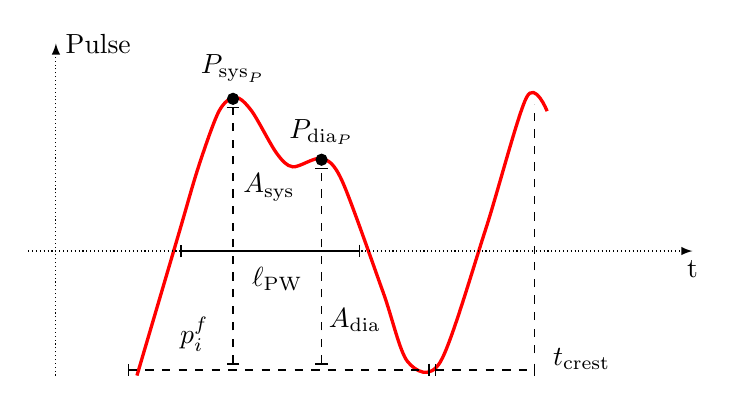
\begin{tikzpicture}
\begin{axis}[
    width=12cm,
    height=6cm,
    xlabel={Time},
    ylabel={mmHg},
    xmin=-5, xmax=15,
    ymin=-10, ymax=15,
    axis lines=none,
    ticks=none,
    every axis plot/.append style={very thick},
    %legend pos=north east
]


    \addplot[red, smooth] coordinates {
         (-1,-10) (0,0) (0.5,5) (1, 9) (1.4,10) (1.8,9) (2.4,6) (2.8,5) (3.5,5.6) (4,4) (5,-4) (5.6,-9) (6.4,-9) (7.5,0.5) (8.5,10) (9,9)
    };
    %\addlegendentry{Second Quadratic}
    \draw[|-|,dashed, left] (94pt,4pt) -- (94pt,97pt);
    \node at (107pt,68pt) [black] {$A_{\mathrm{sys}}$};
    \draw[|-|,dashed, left] (126pt,4pt) -- (126pt,75pt);
    \node at (138pt,20pt) [black] {$A_{\mathrm{dia}}$};
    \draw[|-|,dashed, left] (56pt,2pt) -- (165pt,2pt);
    \node at (80pt,15pt) [black] {$p_i^f$};
    \draw[|-|,dashed, left] (167pt,2pt) -- (203pt,2pt);
    \node at (220pt,6pt) [black] {$t_{\mathrm{crest}}$};
    \draw[dashed, left] (203pt,8pt) -- (203pt,98pt);
    \draw[|-|, left] (75pt,45pt) -- (140pt,45pt);
    \node at (110pt,35pt) [black] {$\ell_{\mathrm{PW}}$};
    \draw[fill=black] (94pt,100pt) circle (2pt);
    \node at (94pt,111pt) [black] {$P_{{\mathrm{sys}_{P}}}$};
    \draw[fill=black] (126pt,78pt) circle (2pt);
    \node at (126pt,88pt) [black] {$P_{{\mathrm{dia}_{P}}}$};

    %axis
    \draw[black, densely dotted, thin, ->] (20pt,45pt) -- (260pt,45pt) node[below] {t};

    \draw[black, densely dotted, thin, ->] (30pt,0pt) -- (30pt,120pt) node[above, right] {Pulse};
\end{axis}
\end{tikzpicture}

\end{document}